 \documentclass[
11pt, % The default document font size, options: 10pt, 11pt, 12pt
% codirector, % Uncomment to add a codirector to the title page
]{charter} 


% El títulos de la memoria, se usa en la carátula y se puede usar el cualquier lugar del documento con el comando \ttitle
\titulo{Implementación de un sistema de bootloader para el SoC SiW G917} 

% Nombre del posgrado, se usa en la carátula y se puede usar el cualquier lugar del documento con el comando \degreename
\posgrado{Carrera de Especialización en Sistemas Embebidos} 
%\posgrado{Carrera de Especialización en Internet de las Cosas} 
%\posgrado{Carrera de Especialización en Inteligencia Artificial}
%\posgrado{Maestría en Sistemas Embebidos} 
%\posgrado{Maestría en Internet de las cosas}
% IMPORTANTE: no omitir titulaciones ni tildación en los nombres, también se recomienda escribir los nombres completos (tal cual los tienen en su documento)
% Tu nombre, se puede usar el cualquier lugar del documento con el comando \authorname
\autor{Ing. Guido Ramírez}

% El nombre del director y co-director, se puede usar el cualquier lugar del documento con el comando \supname y \cosupname y \pertesupname y \pertecosupname
\director{Ms. Jonathan Cagua}
\pertenenciaDirector{Easymetering} 
\codirector{} % para que aparezca en la portada se debe descomentar la opción codirector en los parámetros de documentclass
\pertenenciaCoDirector{FIUBA}

% Nombre del cliente, quien va a aprobar los resultados del proyecto, se puede usar con el comando \clientename y \empclientename
\cliente{Joffre Anzules}
\empresaCliente{Easymetering}
 
\fechaINICIO{20 de agosto de 2024}		%Fecha de inicio de la cursada de GdP \fechaInicioName
\fechaFINALPlan{8 de octubre de 2024} 	%Fecha de final de cursada de GdP
\fechaFINALTrabajo{15 de junio de 2025}	%Fecha de defensa pública del trabajo final


\begin{document}

\maketitle
\thispagestyle{empty}
\pagebreak


\thispagestyle{empty}
{\setlength{\parskip}{0pt}
\tableofcontents{}
}
\pagebreak


\section*{Registros de cambios}
\label{sec:registro}


\begin{table}[ht]
\label{tab:registro}
\centering
\begin{tabularx}{\linewidth}{@{}|c|X|c|@{}}
\hline
\rowcolor[HTML]{C0C0C0} 
Revisión & \multicolumn{1}{c|}{\cellcolor[HTML]{C0C0C0}Detalles de los cambios realizados} & Fecha      \\ \hline
0      & Creación del documento                                 &\fechaInicioName \\ \hline
%1      & Se completa hasta el punto 5 inclusive                & {día} de {mes} de 202X \\ \hline
%2      & Se completa hasta el punto 9 inclusive
%		  Se puede agregar algo más \newline
%		  En distintas líneas \newline
%		  Así                                                    & {día} de {mes} de 202X \\ \hline
%3      & Se completa hasta el punto 12 inclusive                & {día} de {mes} de 202X \\ \hline
%4      & Se completa el plan	                                 & {día} de {mes} de 202X \\ \hline

% Si hay más correcciones pasada la versión 4 también se deben especificar acá

\end{tabularx}
\end{table}

\pagebreak



\section*{Acta de constitución del proyecto}
\label{sec:acta}

\begin{flushright}
Buenos Aires, \fechaInicioName
\end{flushright}

\vspace{2cm}

Por medio de la presente se acuerda con el \authorname\hspace{1px} que su Trabajo Final de la \degreename\hspace{1px} se titulará ``\ttitle'' y consistirá en \textcolor{red}{la implementación de un prototipo de un sistema de control de temperatura de una caldera industrial}. El trabajo tendrá un presupuesto preliminar estimado de \textcolor{red}{600} horas y un costo estimado de \textcolor{red}{\$ XXX}, con fecha de inicio el \fechaInicioName\hspace{1px} y fecha de presentación pública el \fechaFinalName.

Se adjunta a esta acta la planificación inicial.

\vfill

% Esta parte se construye sola con la información que hayan cargado en el preámbulo del documento y no debe modificarla
\begin{table}[ht]
\centering
\begin{tabular}{ccc}
\begin{tabular}[c]{@{}c@{}}Dr. Ing. Ariel Lutenberg \\ Director posgrado FIUBA\end{tabular} & \hspace{2cm} & \begin{tabular}[c]{@{}c@{}}\clientename \\ \empclientename \end{tabular} \vspace{2.5cm} \\ 
\multicolumn{3}{c}{\begin{tabular}[c]{@{}c@{}} \supname \\ Director del Trabajo Final\end{tabular}} \vspace{2.5cm} \\
\end{tabular}
\end{table}




\section{1. Descripción técnica-conceptual del proyecto a realizar}
\label{sec:descripcion}

\section{1.1 Estado del arte}
\label{sec:estadoDelArte}

\section{1.1.1 Bootloader}
\label{sec:edaBootloader}

Un bootloader o arrancador no es diferente a una aplicación cómun en un microcontrolador. De hecho, es igual a una aplicación común. Lo que hace especial a esta es su propósito: permitir la actualización y administración de software sin unar un hardware especializado, y en algunos casos, ser el primer punto de chequeo de integridad de un sistema embebido. Existen variedad de bootloaders; pueden comunicarse a través de diferentes protocolos como UART, CAN, I2C, Ethernet, USB, entre otros. Los sistemas que poseen un arrancador tienen dentro dos programas coexistiendo y deben ser capaces de detectar la existencia de actualizaciones de sistema en progreso.

Cada boootloader puede tener requerimientos únicos basados en su aplicación objetivo, sin embargo existen procesos generales como la capacidad de cambiar entre programa y bootloader, comunicación a través de una interfaz, análisis de registros, guardado de datos en memoria no vólatil, chequeo de integridad de aplicaciones y seguridad del código almacenado.Independientemente de los requerimientos de la aplicación, los procesos generales inducen a una operación relativamente estandar.

En la figura \ref{fig:bootloaderFlow} se puede observar la operación de un bootloader génerico. Se destaca que en el incio del programa se decide correr la aplicación o al arrancador. Este último tiene la capacidad de receptar y ejectuar comandos, y finalmente salir de la aplicación. Los comandos abarcan las operaciones generales mencionadas anteriormente, y pueden añadir el uso de otros periféricos o el envio de datos adicionales hacia un anfitrión.

\begin{figure}[htpb]
\centering 
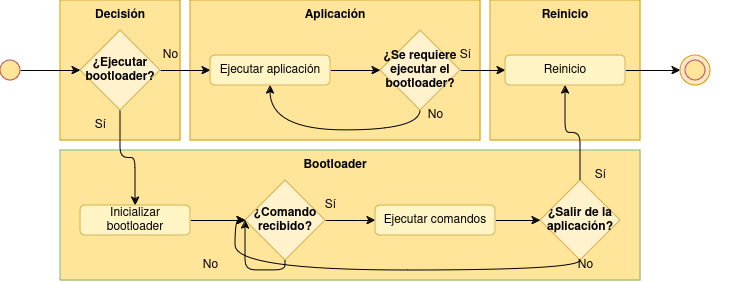
\includegraphics[width=.99\textwidth]{./Figuras/GdP-diagrams-bootloader.png}
\caption{Operación génerica de un bootloader.}
\label{fig:bootloaderFlow}
\end{figure}

\newpage

\section{1.2 Problemática}
\label{sec:s1Problematica}

Easymetering es una empresa que diseña y distribuye módulos AMI (Advanced Metering Infraestructure por sus siglas en inglés). Los módulos AMI son sistemas que miden, recolectan y analizan el uso de la energía, e interactúan con dispositivos como los medidores inteligentes de electricidad, de gas o de agua. Estos son capaces de gestionar información recolectada y tomar deciciones.

Actualmente, ofrecen productos basados en los microcontroladores de los fabricantes Nordic, Microchip, NXP y Espressif. Los módulos AMI, solución más vendida en América latina, usan microcontroladores del último fabricante. Por otro lado, productos usando otras familias se producen o se venden muy poco  .La compañía, con visión de ingresar a otros mercados, ha decidido ampliar su cartera de productos incorporando familias de microcontroladores basados en procesadores ARM Cortex-M a sus módulos AMI. Una de las ventajas de esto, es su escalabilidad, es decir, no se limitan a microcontroladores de bajo costo, sino que los fabricantes han diseñado una serie de soluciones a distintas necesidades. Entre ellas destacan microcontroladores con multiples proccesadores para procesamiento extensivo de señales digitales o datos; sistemas sobre un chip complejos para manejo de energía, sistemas de control, conectividad e internet de las cosas.

Agregar nuevos microcontroladores a la solución AMI de Easymetering, conlleva incorporarlo a su sistema de producción. Este se encarga de guardar información relevante del módulo como seriales del equipo, interfaces de red y periféricos. Actualmente, existe un arrancador o binario de producción que no contempla la inclusión de nuevas familias de microcontroladores y su implementación es bastante especifica para microcontroladores de Espressif. También, existen distintas versiones de arrancador específicos para otras familias. Esto dificulta la incorpración de nuevas solciones o requisitos.  Por ende, se plantea desarrollar un arrancador génerico y portable.

\section{1.3 Solución}
\label{sec:s1Solución}

En el diagrama de descomposición de la figura \ref{fig:sec1BootloaderSolution} se muestra la comunicación entre los módulos para el bootloader génerico propuesto. A pesar de que los procesos generales mostrados al principio de la sección no están explicitamente mencionados, serán considerados en la propuesta. El bootloader será capaz de interactuar con el sistema de producción de la compañía, receptando y ejecutando comandos. Es importante destacar que los módulos a realizar seguirán buenas prácticas de programación, lo que resultará en escalabilidad y portabilidad. 

\begin{figure}[htpb]
\centering 
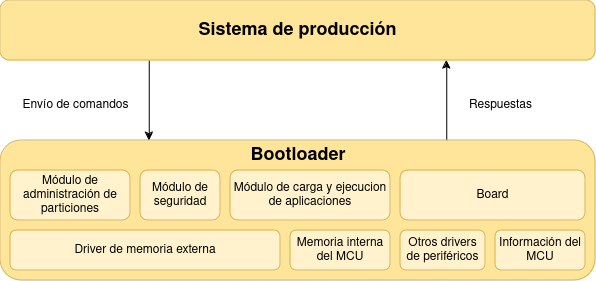
\includegraphics[width=.80\textwidth]{./Figuras/GdPDiagrams-sec1_solution.png}
\caption{Diagrama de bloques de bootloader propuesto.}
\label{fig:sec1BootloaderSolution}
\end{figure}

Los módulos de administración de particiones, seguridad y carga y ejecución de aplicaciones juegan un rol importante para el bootloader. Son los encargados de interactuar con la memoria externa usada e interna del microcontrolador. Las interacciones con la primera son son leer, escribir y borrar aplicaciones. La relación con la memoria del microcontrolador consiste en escribir aplicaciones provenientes de la otra memoria y ejecutarlas cuando se requiera. Por otro lado, el módulo de administración de particiones y seguridad se encargará de dividir la memoria externa y establecer parametros de seguridad para chequear la integridad de sus contenidos. Por último, el módulo de \textit{board} interactua cercanamente con la información proporcionada por \textit{drivers} de otros periféricos y del microcontrolador, con la finalidad de enviar datos relevantes al sistema de producción.

El valor agregado a nuestra propuesta es un bootloader reutilizable y escalable para futuras soluciones que usen otras familias de microcontroladores. Además, cumple con la necesidad especifica de la compañía de un sistema de almacenamiento de binarios propio, con particionamiento y lineamientos de seguridad personalizados.

\newpage

\section{2. Identificación y análisis de los interesados}
\label{sec:interesados}

\begin{table}[ht]
%\caption{Identificación de los interesados}
%\label{tab:interesados}
\begin{tabularx}{\linewidth}{@{}|l|X|X|l|@{}}
\hline
\rowcolor[HTML]{C0C0C0} 
Rol           & Nombre y Apellido & Organización 	& Puesto 	\\ \hline
Auspiciante   &   -               &     -         	&    -    	\\ \hline
Cliente       & \clientename      &\empclientename	&    Gerente General    \\ \hline
Impulsor      &      -             &      -        	&     -   	\\ \hline
Responsable   & \authorname       & FIUBA        	& Alumno 	\\ \hline
Colaboradores &      -             &     -         	&     -   	\\ \hline
Orientador    & \supname	      & \pertesupname 	& Director del Trabajo Final \\ \hline
Equipo        & 	 -             &      -       	&       - 	\\ \hline
Opositores    &      -             &      -        	&       - 	\\ \hline
Usuario final &      -             &      -        	&       - 	\\ \hline
\end{tabularx}
\end{table}

\begin{itemize}
	\item Orientador: El \supname\  tiene una larga trayectoria como desarrollador de firmware y hardware. Tiene experiencia usando varios microcontroladores incluyendo el seleccionado para este proyecto.
\end{itemize}

\section{3. Propósito del proyecto}
\label{sec:proposito}


El próposito del proyecto es desarrollar un \textit{bootloader} portable para distintas familias de microcontroladores, inicialmente dirigido hacia el SoC SiW G917. El proyecto nace de la integración de nuevos productos basados en otras familias de microprocesadores con el objetivo de ofrecerlos e implementarlos en otros mercados. El \textit{bootloader} debe acoplarse al sistema de producción actual de la compañía. El arrancador usa una memoria externa particionada con lineamientos de seguridad establecidos por el cliente; almacena y administra aplicaciones binarias. Además, se comunica con el sistema de producción a través de una computadora anfitriona para ejecutar comandos y almacenar datos relevantes del equipo. 

\section{4. Alcance del proyecto}
\label{sec:alcance}

El proyecto incluye:
\begin{itemize}
	\item Desarrollo del driver para el manejo de memoria flash externa.
	\item Diseño de particiones de la memoria flash externa.
	\item Manejo de archivos \textit{linker} del microcontrolador.
	\item Integración de capas de seguridad en las imágenes del dispositivo.
	\item Integración con el sistema de producción de la empresa
		\begin{itemize}
		\item Comunicación serial.
		\item Control de versiones de hardware.
		\item Control de versiones de firmware.
		\item Control de inventario.
		\end{itemize}	
\end{itemize}

El proyecto no incluye:
\begin{itemize}
	\item Diseño de hardware.
	\item Comunicación wi-fi con el sistema de producción.
\end{itemize}

\section{5. Supuestos del proyecto}
\label{sec:supuestos}

Para el desarrollo del presente proyecto se cuenta con:

\begin{itemize}
	\item Existencias dentro de la compañía del integrado \textit{W25Q64JVZPIQTR}, memoria flash externa.
	\item Disponibilidad de una placa de desarrollo basada en el SoC objetivo.
	\item Una computadora para el desarrollo del proyecto.
	\item Disponibilidad del equipo de backend para consultas sobre el sistema de producción.
\end{itemize}

\section{6. Requerimientos}
\label{sec:requerimientos}

\begin{enumerate}
	\item Requerimientos funcionales:
		\begin{enumerate}
			
			\item La placa debe acoplarse al sistema de producción de la empresa.
			\item La placa debe guardar los datos de producción de la compañía.
			\item El usuario puede cargar distintos binarios a la placa objetivo.
			\item El usuario puede arrancar cualquier binario cargado a la placa objetivo.
			\item El sistema debe poder volver al bootloader.
			\item El sistema detecta cuando hubo una actualización de binarios.
			\item Los binarios almacenados no son guardados en texto plano.
			\item Los binarios, antes de ser almacenados, son encriptados usando el módulo de seguridad del sistema.
		\end{enumerate}
	\item Requerimientos de documentación:
		\begin{enumerate}
			\item Documentación usando Doxygen en todos los módulos, componentes o drivers
			\item Documento de la materia 'Gestión de Proyectos'.
			\item Documento de la memoria técnica.
		\end{enumerate}
	\item Requerimiento de testing:
		\begin{enumerate}
			\item Testing de driver para memoria externa.
			\item Testing de driver para consola.
			\item Testing de administración de particiones.
			\item Testing de módulo de seguridad.
			\item Testing de componente board.
		\end{enumerate}
	\item Requerimientos de la interfaz:
		\begin{enumerate}
			\item Imitar el sistema de producción para prueba de concepto.
		\end{enumerate}
\end{enumerate}

\section{7. Historias de usuarios (\textit{Product backlog})}
\label{sec:backlog}

A continuación, se dan a conocer historias de usarios valoradas con \textit{story points}, basados en tres categorías aplicadas en cada historia: dificultad, D; complejidad, C; y riesgo, R. Cada categoría tiene asignada tres niveles: bajo, medio y alto. Cada nivel es asociado con un puntaje de 1, 2 y 3 respectivamente. Finalmente, se suman los niveles asignados a cada categoría para obtener la valoración final de la historia. Si la valoración no es un número de la serie Fibonacci, entonces se aproxima al número superior más cercano de la secuencia. El resultado nos informa de la dificultad, complejidad y riesgo del trabajo a realizar para cada historia de usuario.

\begin{itemize}
	\item "Como miembro del departamento de firmware, espero que el bootloader de nuestros equipos sea escalable para incorporar nuevas tecnologías o requerimientos, con la finalidad de trabajar o dar mantenimiento a un único proyecto de software"
	\begin{itemize}
		\item D:3 + C:3 + R:2 $\rightarrow$ 8
	\end{itemize}
	\item "Como miembro del departamento de firmware, es viable tener un sistema de arranque y administración de binarios genérico, para mantener nuestro código reutilizable y escalable"
	\begin{itemize}
		\item D:3 + C:2 + R:1 $\rightarrow$ 8
	\end{itemize}
	\item "Como encargado del departamento de producción, me interesa que nuevos productos sean incorporados fácilmente en nuestra base de datos, para minimizar el tiempo empleado en cada orden"
	\begin{itemize}
		\item D:2 + C:2 + R:1 $\rightarrow$ 5
	\end{itemize}
	\item "Como encargado del departamento de producción, quiero manejar una única versión actualizada de bootloader, para poder cargar binarios de aplicación para distintas soluciones o productos."
	\begin{itemize}
		\item D:3 + C:3 + R:3 $\rightarrow$ 13
	\end{itemize}
	\item "Como CEO de Easymetering, deseo a futuro delegar ordenes de producción grandes de nuestras soluciones a las fabricas ensambladoras, con un bootloader que siga nuestros lineamientos de seguridad y encriptación, para evitar la filtración de nuestros binarios de aplicación."
	\begin{itemize}
		\item D:1 + C:3 + R:3 $\rightarrow$ 8
	\end{itemize}
\end{itemize}

\section{8. Entregables principales del proyecto}
\label{sec:entregables}

Los entregables del proyecto son:

\begin{itemize}
	\item Documentación usando doxygen.
	\item Documentación de la partición de memoria externa usada.
	\item Diagrama de flujo de procesos relevantes.
	\item Código fuente del firmware para módulos, componentes o drivers.
	\item La placa objetivo es agregada al sistema de producción.
	\item Memoria del trabajo final.
\end{itemize}

\section{9. Desglose del trabajo en tareas}
\label{sec:wbs}

En esta sección se desglosa el trabajo a realizar en una lista de tareas generales y específicas.

\begin{enumerate}
\item Familiarizarse con placa objetivo (64 h)
	\begin{enumerate}
	\item Leer datasheets del SoC (4 h)
	\item Leer guias para desarrolladores del IDE (10 h)
	\item Familiarizarse con IDE (20 h)
	\item Familiarizarse con el SDK del fabricante (20 h)
	\item Familiarizarse con ambiente de configuración del fabricante (10 h)
	\end{enumerate}
\item Módulo de consola (32 h)
	\begin{enumerate}
	\item Diseño de módulo (8 h)
	\item Implementación de funciones (8 h)
	\item Testing (8 h)
	\item Pruebas (8 h)
	\end{enumerate}
\item Protocolo de sistema de producción (66 h)
	\begin{enumerate}
	\item Diseñar módulo para protocolo (8 h)
	\item Implementar funciones (16 h)
	\item Ejecutar comandos (24 h)
	\item Testing (8 h)
	\item Pruebas (8 h)
	\end{enumerate}
\item Driver memoria externa (52 h)
	\begin{enumerate}
	\item Leer documentación del integrado (4 h)
	\item Diseño del driver	(8 h)
	\item Implementación de funciones (24 h)
	\item Testing (8 h)
	\item Pruebas (8 h)
	\end{enumerate}
\item Módulo de seguridad (50 h)
	\begin{enumerate}
	\item Investigación de algoritmos usados en trabajos anteriores (8 h)
	\item Definir algoritmos a usar (8 h)
	\item Investigar librería de algoritmos disponible (8 h)
	\item Implementación de funciones (16 h)
	\item Testing (8 h)
	\end{enumerate}
\item Módulo de administración de particiones (80 h)
	\begin{enumerate}
	\item Investigación y diseño de control particiones (24 h)
	\item Diseño de cabecera para binarios (8 h)
	\item Diseño de información de producción guardada (8 h)
	\item Implementación de funciones (24 h)
	\item Testing  (8 h)
	\item Pruebas  (8 h)
	\end{enumerate}
\item Módulo de carga y ejecución de aplicaciones (80 h)
	\begin{enumerate}
	\item Investigar funcionamiento memoria en la palca (20 h)
	\item Diseño de módulo (20 h)
	\item Implementación de funciones (24 h)
	\item Testing (8 h)
	\item Pruebas (12 h)
	\end{enumerate}
\item Módulo de board (64 h)
	\begin{enumerate}
	\item Investigar módulos de board de otros fabricantes (8 h)
	\item Diseño del módulo (8 h)
	\item Diseño de cabecera para binarios (8 h)
	\item Implementación de funciones (24 h)
	\item Testing  (8 h)
	\item Pruebas  (8 h)
	\end{enumerate}
\item Documento 'Gestión de proyectos' (20 h)
	\begin{enumerate}
	\item Realizar documento (20 h)
	\end{enumerate} 
\item Documento memoria técnica (80 h)
	\begin{enumerate}
	\item Taller de trabajo final A (40 h)
	\item Taller de trabajo final B (40 h)
	\end{enumerate} 
\end{enumerate}

Cantidad total de horas: 588 h.

\section{10. Diagrama de Activity On Node}
\label{sec:AoN}

\begin{consigna}{red}
Armar el AoN a partir del WBS definido en la etapa anterior.

Una herramienta simple para desarrollar los diagramas es el Draw.io (\url{https://app.diagrams.net/}).
\href{https://app.diagrams.net}{Draw.io}


\begin{figure}[htpb]
\centering 
\includegraphics[width=.8\textwidth]{./Figuras/AoN.png}
\caption{Diagrama de \textit{Activity on Node}.}
\label{fig:AoN}
\end{figure}

Indicar claramente en qué unidades están expresados los tiempos.
De ser necesario indicar los caminos semi críticos y analizar sus tiempos mediante un cuadro.
Es recomendable usar colores y un cuadro indicativo describiendo qué representa cada color.

\end{consigna}

\section{11. Diagrama de Gantt}
\label{sec:gantt}

\begin{consigna}{red}
Existen muchos programas y recursos \textit{online} para hacer diagramas de Gantt, entre los cuales destacamos:

\begin{itemize}
\item Planner
\item GanttProject
\item Trello + \textit{plugins}. En el siguiente link hay un tutorial oficial: \\ \url{https://blog.trello.com/es/diagrama-de-gantt-de-un-proyecto}
\item Creately, herramienta online colaborativa. \\\url{https://creately.com/diagram/example/ieb3p3ml/LaTeX}
\item Se puede hacer en latex con el paquete \textit{pgfgantt}\\ \url{http://ctan.dcc.uchile.cl/graphics/pgf/contrib/pgfgantt/pgfgantt.pdf}
\end{itemize}

Pegar acá una captura de pantalla del diagrama de Gantt, cuidando que la letra sea suficientemente grande como para ser legible. 
Si el diagrama queda demasiado ancho, se puede pegar primero la ``tabla'' del Gantt y luego pegar la parte del diagrama de barras del diagrama de Gantt.

Configurar el software para que en la parte de la tabla muestre los códigos del EDT (WBS).\\
Configurar el software para que al lado de cada barra muestre el nombre de cada tarea.\\
Revisar que la fecha de finalización coincida con lo indicado en el Acta Constitutiva.

En la figura \ref{fig:gantt}, se muestra un ejemplo de diagrama de gantt realizado con el paquete de \textit{pgfgantt}. 
En la plantilla pueden ver el código que lo genera y usarlo de base para construir el propio.

Las fechas pueden ser calculadas utilizando alguna de las herramientas antes citadas. Sin embargo, el siguiente ejemplo
fue elaborado utilizando 
\href{https://docs.google.com/spreadsheets/d/1fBz8NhSpc4tkkhz3KjJCbh1nR_ltDkfEcZi4tZXduqs}{esta hoja de cálculo}.

Es importante destacar que el ancho del diagrama estará dado por la longitud del texto utilizado para las tareas 
(Ejemplo: tarea 1, tarea 2, etcétera) y el valor \textit{x unit}. Para mejorar la apariencia del diagrama, es necesario
ajustar este valor y, quizás, acortar los nombres de las tareas.

\begin{figure}[htpb]
  \begin{center}
    \begin{ganttchart}[
      time slot unit=day,
      time slot format=isodate,
      x unit=0.038cm,
      y unit title=0.7cm,
      y unit chart=0.6cm,
      milestone/.append style={xscale=4}
      ]{2021-03-05}{2021-12-16}
      \gantttitlecalendar*{2021-03-05}{2021-12-16}{year} \\
      \gantttitlecalendar*{2021-03-05}{2021-12-16}{month} \\
      \ganttgroup{Duración Total}{2021-03-05}{2021-12-16} \\
      %%%%%%%%%%%%%%%%%Organización
      \ganttgroup{Organización}{2021-03-05}{2021-04-16} \\
      \ganttbar{Planificación del proyecto}{2021-03-05}{2021-04-15} \\
      %%%%%%%%%%%%%%%%%Ejecución
      \ganttgroup{Ejecución}{2021-04-16}{2021-10-21} \\
      \ganttbar{Tarea 1}{2021-04-16}{2021-04-29} \\
      \ganttbar{Tarea 2}{2021-04-30}{2021-05-13} \\
      \ganttbar{Tarea 3}{2021-05-14}{2021-05-27} \\
      \ganttbar{Tarea 4}{2021-05-28}{2021-07-12} \\
      \ganttbar{Tarea 5}{2021-07-13}{2021-08-09} \\
      \ganttbar{Tarea 6}{2021-08-10}{2021-09-23} \\
      \ganttbar{Tarea 7}{2021-09-24}{2021-09-30} \\
      \ganttbar{Tarea 8}{2021-10-01}{2021-10-14} \\
      \ganttbar{Tarea 9}{2021-10-15}{2021-10-21} \\
      % %%%%%%%%%%%%%%%%%Finalización
      \ganttgroup{Finalización}{2021-10-22}{2021-12-16} \\
      \ganttbar{Memoria v1}{2021-10-22}{2021-11-04} \\
      \ganttbar{Memoria v2}{2021-11-05}{2021-11-18} \\
      \ganttbar{Memoria final}{2021-11-19}{2021-12-02} \\
      % La fecha del siguiente milestone es la fecha en que terminamos la memoria
      \ganttmilestone{Enviar memoria al director}{2021-12-02} \\
      \ganttbar{Elaborar la presentación}{2021-12-03}{2021-12-16} \\
      \ganttmilestone{Ensayo de la presentación}{2021-12-16} \\
      %%%%%%%%%%%%%%%%%%%%%%%%%%%%%%%%%%%%%%%%%%%%%%%%%%%%%%%%%%%%%%%
    \end{ganttchart}
  \end{center}
  \caption{Diagrama de gantt de ejemplo}
  \label{fig:gantt}
\end{figure}


\begin{landscape}
\begin{figure}[htpb]
\centering 
\includegraphics[height=.85\textheight]{./Figuras/Gantt-2.png}
\caption{Ejemplo de diagrama de Gantt (apaisado).} %Modificar este título acorde.
\label{fig:diagGantt}
\end{figure}

\end{landscape}

\end{consigna}


\section{12. Presupuesto detallado del proyecto}
\label{sec:presupuesto}

\begin{consigna}{red}
Si el proyecto es complejo entonces separarlo en partes:
\begin{itemize}
	\item Un total global, indicando el subtotal acumulado por cada una de las áreas.
	\item El desglose detallado del subtotal de cada una de las áreas.
\end{itemize}

IMPORTANTE: No olvidarse de considerar los COSTOS INDIRECTOS.

Incluir la aclaración de si se emplea como moneda el peso argentino (ARS) o si se usa moneda extranjera (USD, EUR, etc). Si es en moneda extranjera se debe indicar la tasa de conversión respecto a la moneda local en una fecha dada.

\end{consigna}

\begin{table}[htpb]
\centering
\begin{tabularx}{\linewidth}{@{}|X|c|r|r|@{}}
\hline
\rowcolor[HTML]{C0C0C0} 
\multicolumn{4}{|c|}{\cellcolor[HTML]{C0C0C0}COSTOS DIRECTOS} \\ \hline
\rowcolor[HTML]{C0C0C0} 
Descripción &
  \multicolumn{1}{c|}{\cellcolor[HTML]{C0C0C0}Cantidad} &
  \multicolumn{1}{c|}{\cellcolor[HTML]{C0C0C0}Valor unitario} &
  \multicolumn{1}{c|}{\cellcolor[HTML]{C0C0C0}Valor total} \\ \hline
 &
  \multicolumn{1}{c|}{} &
  \multicolumn{1}{c|}{} &
  \multicolumn{1}{c|}{} \\ \hline
 &
  \multicolumn{1}{c|}{} &
  \multicolumn{1}{c|}{} &
  \multicolumn{1}{c|}{} \\ \hline
\multicolumn{1}{|l|}{} &
   &
   &
   \\ \hline
\multicolumn{1}{|l|}{} &
   &
   &
   \\ \hline
\multicolumn{3}{|c|}{SUBTOTAL} &
  \multicolumn{1}{c|}{} \\ \hline
\rowcolor[HTML]{C0C0C0} 
\multicolumn{4}{|c|}{\cellcolor[HTML]{C0C0C0}COSTOS INDIRECTOS} \\ \hline
\rowcolor[HTML]{C0C0C0} 
Descripción &
  \multicolumn{1}{c|}{\cellcolor[HTML]{C0C0C0}Cantidad} &
  \multicolumn{1}{c|}{\cellcolor[HTML]{C0C0C0}Valor unitario} &
  \multicolumn{1}{c|}{\cellcolor[HTML]{C0C0C0}Valor total} \\ \hline
\multicolumn{1}{|l|}{} &
   &
   &
   \\ \hline
\multicolumn{1}{|l|}{} &
   &
   &
   \\ \hline
\multicolumn{1}{|l|}{} &
   &
   &
   \\ \hline
\multicolumn{3}{|c|}{SUBTOTAL} &
  \multicolumn{1}{c|}{} \\ \hline
\rowcolor[HTML]{C0C0C0}
\multicolumn{3}{|c|}{TOTAL} &
   \\ \hline
\end{tabularx}%
\end{table}


\section{13. Gestión de riesgos}
\label{sec:riesgos}

\begin{consigna}{red}
a) Identificación de los riesgos (al menos cinco) y estimación de sus consecuencias:
 
Riesgo 1: detallar el riesgo (riesgo es algo que si ocurre altera los planes previstos de forma negativa)
\begin{itemize}
	\item Severidad (S): mientras más severo, más alto es el número (usar números del 1 al 10).\\
	Justificar el motivo por el cual se asigna determinado número de severidad (S).
	\item Probabilidad de ocurrencia (O): mientras más probable, más alto es el número (usar del 1 al 10).\\
	Justificar el motivo por el cual se asigna determinado número de (O). 
\end{itemize}   

Riesgo 2:
\begin{itemize}
	\item Severidad (S): X.\\
	Justificación...
	\item Ocurrencia (O): Y.\\
	Justificación...
\end{itemize}

Riesgo 3:
\begin{itemize}
	\item Severidad (S):  X.\\
	Justificación...
	\item Ocurrencia (O): Y.\\
	Justificación...
\end{itemize}


b) Tabla de gestión de riesgos:      (El RPN se calcula como RPN=SxO)

\begin{table}[htpb]
\centering
\begin{tabularx}{\linewidth}{@{}|X|c|c|c|c|c|c|@{}}
\hline
\rowcolor[HTML]{C0C0C0} 
Riesgo & S & O & RPN & S* & O* & RPN* \\ \hline
       &   &   &     &    &    &      \\ \hline
       &   &   &     &    &    &      \\ \hline
       &   &   &     &    &    &      \\ \hline
       &   &   &     &    &    &      \\ \hline
       &   &   &     &    &    &      \\ \hline
\end{tabularx}%
\end{table}

Criterio adoptado: 

Se tomarán medidas de mitigación en los riesgos cuyos números de RPN sean mayores a...

Nota: los valores marcados con (*) en la tabla corresponden luego de haber aplicado la mitigación.

c) Plan de mitigación de los riesgos que originalmente excedían el RPN máximo establecido:
 
Riesgo 1: plan de mitigación (si por el RPN fuera necesario elaborar un plan de mitigación).
  Nueva asignación de S y O, con su respectiva justificación:
  \begin{itemize}
	\item Severidad (S*): mientras más severo, más alto es el número (usar números del 1 al 10).
          Justificar el motivo por el cual se asigna determinado número de severidad (S).
	\item Probabilidad de ocurrencia (O*): mientras más probable, más alto es el número (usar del 1 al 10).
          Justificar el motivo por el cual se asigna determinado número de (O).
	\end{itemize}

Riesgo 2: plan de mitigación (si por el RPN fuera necesario elaborar un plan de mitigación).
 
Riesgo 3: plan de mitigación (si por el RPN fuera necesario elaborar un plan de mitigación).

\end{consigna}


\section{14. Gestión de la calidad}
\label{sec:calidad}

\begin{consigna}{red}
Elija al menos diez requerimientos que a su criterio sean los más importantes/críticos/que aportan más valor y para cada uno de ellos indique las acciones de verificación y validación que permitan asegurar su cumplimiento.

\begin{itemize} 
\item Req \#1: copiar acá el requerimiento con su correspondiente número.

\begin{itemize}
	\item Verificación para confirmar si se cumplió con lo requerido antes de mostrar el sistema al cliente. Detallar.
	\item Validación con el cliente para confirmar que está de acuerdo en que se cumplió con lo requerido. Detallar. 
\end{itemize}

\end{itemize}

Tener en cuenta que en este contexto se pueden mencionar simulaciones, cálculos, revisión de hojas de datos, consulta con expertos, mediciones, etc.  

Las acciones de verificación suelen considerar al entregable como ``caja blanca'', es decir se conoce en profundidad su funcionamiento interno.  

En cambio, las acciones de validación suelen considerar al entregable como ``caja negra'', es decir, que no se conocen los detalles de su funcionamiento interno.

\end{consigna}

\section{15. Procesos de cierre}    
\label{sec:cierre}

\begin{consigna}{red}
Establecer las pautas de trabajo para realizar una reunión final de evaluación del proyecto, tal que contemple las siguientes actividades:

\begin{itemize}
	\item Pautas de trabajo que se seguirán para analizar si se respetó el Plan de Proyecto original:\\
	 - Indicar quién se ocupará de hacer esto y cuál será el procedimiento a aplicar. 
	\item Identificación de las técnicas y procedimientos útiles e inútiles que se emplearon, los problemas que surgieron y cómo se solucionaron:\\
	 - Indicar quién se ocupará de hacer esto y cuál será el procedimiento para dejar registro.
	\item Indicar quién organizará el acto de agradecimiento a todos los interesados, y en especial al equipo de trabajo y colaboradores:\\
	  - Indicar esto y quién financiará los gastos correspondientes.
\end{itemize}

\end{consigna}

\end{document}